% --- INICIO DE PLANTILLA PERSONALIZADA ---
\documentclass[oneside,11pt]{Latex/Classes/PhDthesisPSnPDF}

% --- Paquetes Originales ---
\usepackage{blindtext}
\usepackage{actuarialangle} 
\usepackage{tabularx}
\usepackage{float}
\usepackage{multirow, array}
\usepackage[usenames,dvipsnames,svgnames,table]{xcolor}
\usepackage{longtable}
\usepackage{latexsym,amsmath,amssymb,amsfonts}
\usepackage{enumitem}
\usepackage{xparse}
\usepackage{booktabs}
\usepackage[round, sort, numbers]{natbib}  
\usepackage{adjustbox}
\usepackage[utf8]{inputenc}
\usepackage{caption}
\usepackage{graphicx}
\usepackage{hyperref}
\usepackage{cleveref}

% Definición de colores
\definecolor{miblue}{RGB}{68, 114, 196}

% --- CAMBIO CRÍTICO 1: Usar \input para macros en el preámbulo ---
% \include da problemas antes del begin document. \input es seguro.
\input{Latex/Macros/MacroFile1}

% --- Definiciones de seguridad (por si la clase falla al cargar alguna variable) ---
\providecommand{\facultad}[1]{\def\lafacultad{#1}}
\providecommand{\escudofacultad}[1]{\def\elescudo{#1}}
\providecommand{\degree}[1]{\def\elgrado{#1}}
\providecommand{\director}[1]{\def\eldirector{#1}}
\providecommand{\lugar}[1]{\def\ellugar{#1}}
\providecommand{\degreedate}[1]{\def\lafecha{#1}}

% --- Configuración para bloques de código de R (Pandoc) ---

%%%%%%%%%%%%%%%%%%%%%%%%%%%%%%%%%%%%%%%%%%%%%%%%%%%%%%%%%%%%%%%%%%%%%%%%%%%%%%%%
%                         DATOS (Conectados a RMarkdown)                       %
%%%%%%%%%%%%%%%%%%%%%%%%%%%%%%%%%%%%%%%%%%%%%%%%%%%%%%%%%%%%%%%%%%%%%%%%%%%%%%%%
\title{Estandarización en las canciones con sellos de grandes
discográficas en el género Pop}
\author{Sebastian Soto \\ Valeria Ruza \\ Gabriel Ugas}

% Lógica para Facultad: Si la defines en el YAML la usa, si no, usa la default

\facultad{Facultad de Ciencias Económicas y Sociales \\ Escuela de
Estadistica y Ciencias Actuariales}
  \escudofacultad{Latex/Classes/Escudos/faces}

\degree{Computación I}
\director{Jesus Ochoa \\ Oliver Triveño}
\degreedate{Marzo 2026} 
\lugar{Caracas}

\portadatrue 

% Metadatos PDF
\keywords{}
\subject{}

% --- CORRECCIÓN PARA PANDOC NUEVO (Imágenes) ---
\makeatletter
\providecommand{\pandocbounded}[1]{#1}
\makeatother


%%%%%%%%%%%%%%%%%%%%%%%%%%%%%%%%%%%%%%%%%%%%%%%%%%%%%
%                   DOCUMENTO                       %
%%%%%%%%%%%%%%%%%%%%%%%%%%%%%%%%%%%%%%%%%%%%%%%%%%%%%
\begin{document}

\maketitle

%%%%%%%%%%%%%%%%%%%%%%%%%%%%%%%%%%%%%%%%%%%%%%%%%%%%%
%                  PRÓLOGO                          %
%%%%%%%%%%%%%%%%%%%%%%%%%%%%%%%%%%%%%%%%%%%%%%%%%%%%%
\frontmatter

% Puedes agregar dedicatorias desde el YAML si quieres, o dejarlas fijas aquí

%%%%%%%%%%%%%%%%%%%%%%%%%%%%%%%%%%%%%%%%%%%%%%%%%%%%%
%                   ÍNDICES                         %
%%%%%%%%%%%%%%%%%%%%%%%%%%%%%%%%%%%%%%%%%%%%%%%%%%%%%
\setcounter{secnumdepth}{3}
\setcounter{tocdepth}{3}

\tableofcontents



\cleardoublepage

  \cleardoublepage       % Empieza en página derecha (estándar en tesis)
  \chapter*{Resumen}     % Crea el título "Resumen" sin numeración (Capítulo *)
  \addcontentsline{toc}{chapter}{Resumen} % (Opcional) Lo añade al índice
  
  El proyecto pretende atender al problema de la estandarización en las
canciones con sello de grandes discográficas del género Pop, que afectan
negativamente a la nueva generación, enfocados en la parte estadística
del mismo, analizando las características de las canciones del género
Pop usando como referencia el dataset (Spotify 2015-2025)

El objetivo es comprobar que existe las estandarización en las
características musicales y sonoras de las canciones con sello de
grandes discográficas del género Pop. Y para ello hay que Observar
mediante las variables stream counts y label las discográficas más
exitosas, para tratar los datos en torno a las 3 primeras Discográficas,
luego se toman en cuenta varias variables en este caso:(loudness,
energy, duration ms, instrumentales, explicit, tempo, danceability, key
y mode), se dividen en dos categorías sonoras y musicales, se analizan
las variables de cada categoría aparte usando métodos de dispersión,
distribución y correlación y se explican en histogramas de frecuencias
para las variables dicotómicas, histogramas con curvas de KDE para la
curtosis y ver si se asemejan a una campana de Gauss y por último
gráficas de calor para contemplar la correlación y ver si es alta o
baja. Por último se analizan todos los resultados y se determinaría si
son o no estandarizadas las canciones, luego en caso de ser así se
contemplaría el comportamiento
estándar.             % Aquí se pega el texto que escribiste en el YAML
  
  \cleardoublepage

%%%%%%%%%%%%%%%%%%%%%%%%%%%%%%%%%%%%%%%%%%%%%%%%%%%%%
%                   CONTENIDO (El Corazón)          %
%%%%%%%%%%%%%%%%%%%%%%%%%%%%%%%%%%%%%%%%%%%%%%%%%%%%%
\mainmatter
\def\baselinestretch{1.5}

% --- CAMBIO CRÍTICO 2: Aquí RMarkdown inyecta todo tu texto ---
\chapter*{Introducción}

La industria musical contemporánea se caracteriza por el dominio
oligopólico de grandes discográficas, que controlan la mayoría del
mercado pop global. Este proyecto investiga la hipótesis de que estas
``majors'' promueven una estandarización de las características
musicales, limitando la diversidad sonora disponible para el público
juvenil.

A través del análisis estadístico descriptivo del dataset
\textbf{\emph{Spotify 2015-2025}}, se examinan variables técnicas
(loudness, energy, duration) y estructurales (tempo, danceability, key,
mode) de canciones pop con sello de estas discográficas. El objetivo es
determinar, mediante análisis de dispersión, distribución y correlación,
si existe una homogeneización sistemática en las producciones
comerciales que pudiera condicionar los patrones de consumo y la
creatividad musical actual.

\chapter{Planteamiento del Problema}

Desde finales de los sesenta, cuando se habla de ``Pop'' se refiere,
sobre todo, a la música orientada al consumo rápido y dirigida a los
jóvenes. Canciones de duración corta con ritmos contagiosos, para
alcanzar un éxito popular y comercial dirigido a la mayor cantidad de
público posible y jóvenes. Como escribe John Seabrook ``La fábrica de
canciones. Cómo se hacen los hits''.

Ya que el Pop absorbe características de otros géneros para mantener su
éxito y recurre a letras y melodías repetitivas, románticas y
melancólicas. Esta tendencia cambiante e imitadora, junto con que esté
dirigido a una cantidad de público muy extensa y sobre todo enfocado en
Jóvenes. Influye profundamente en la forma de pensar, sentir y
comportarse de gran parte de la población y los adolescentes, a menudo
fomentando la imitación, según apuntan International Journal of Arts \&
Education Research.

``\,``También, la industria musical es posiblemente uno de los mercados
más competitivos. Los sellos discográficos son empresas que contratan
artistas, financian grabaciones, comercializan la música y coordinan la
distribución. Según una investigación presentada por Juan Francisco
Peñaloza Cubillos, de la Pontificia Universidad Javeriana, concluye que
el mercado musical es un oligopolio entre las grandes compañías
discográficas''\,``.

``actualmente la industria de la música es controlada por tres grandes
compañías discográficas multinacionales también llamadas majors, tanto a
nivel internacional como a nivel nacional, siendo Sony Music, Universal
Music Group y Warner Music Group los que lideran el mercado mundial de
la industria de la música, como también a la gran mayoría de sus
artistas.''

Entonces tomando en cuenta el hecho que el género Pop influencia en la
manera de pensar de los jóvenes y que las discográficas dominan el
mercado, Podemos decir que las canciones con sellos de grandes
discográficas pueden controlar la forma de pensar de los Jóvenes y por
consiguiente si las grandes discográficas tienden a estandarizar las
características sonoras y métricas de las canciones, están imponiendo al
público Juvenil un modelo único de consumo, lo que los lleva a tener
limitaciones en el acceso a la diversidad musical y a la imitación
pasiva.\\

Argumento final. Debido a esto, se plantea las siguientes preguntas de
investigación:\\

\textbf{1.} ¿Qué discográficas son más exitosas según el dataset?\\

\textbf{2.} ¿Las variables analizadas demuestran un comportamiento
similar a lo largo del tiempo, con lo que podemos determinar que las
grandes disqueras musicales comercializan canciones estandarizadas?\\

\textbf{3.} ¿Qué comportamiento demuestran las variables
estandarizadas?\\

\section{Justificación}

Este problema, que relaciona dos temas diferentes nos permite como
estadísticos aplicar el conocimiento del área de Estadística I, como lo
es la estadística descriptiva (Gráficas, Histogramas, matices de
correlación, coeficiente de variación), a través de los lenguajes
estudiado en Computación I como lo es R, aplicando el filtrado y
limpieza del dataset, aplicación de funciones matemáticas y creación de
gráficas, todo en una investigación que se puede adaptar a la
realidad.\\

\section{Objetivos}

\subsection{Objetivo General}
\begin{itemize}
  \item{ Estudiar si las canciones con sellos de grandes discográficas tienden a unas características musicales estandarizadas. (Mediante análisis de dispersión, de distribución y correlación)}
\end{itemize}

\subsection{Objetivos Específicos}
\begin{itemize}
  \item{Analizar qué discográficas son más exitosas: Con la variable Label y Stream count.}
  \item{Adaptar el dataset con los datos de las tres primeras discográficas más exitosas.}
  \item{Categorizar las variables: Para intuir con qué método analizar cada variable, se diferencian por categorías.(Técnicas y sonoras)}
  \item{Analizar las variables técnicas y de producción: Mediante una gráfica de frecuencias para la variable explicit, mediante el coeficiente de variación y un histograma con curva KDE  para loudness, energy, duration, instrumentalness y un mapa de calor para ver la correlación entre todas.}
  \item{Analizar las variables de estructura musical(sonoras): Mediante una gráfica de frecuencias para la variable mode y key, mediante el coeficiente de variación y un histograma con curva KDE  para tempo y danceability y un mapa de calor para ver la correlación entre todas.}
  \item{Analizar los resultados obtenidos y ver si son variables estandarizadas o no y el comportamiento que siguen.}
\end{itemize}

\section{Cobertura}

\subsection{Horizontal}

La cobertura horizontal abarca las características musicales que
componene cada canción\\

\subsection{Vertical}

La cobertura vertical abarca los 85.000 datos del dataset, que son las
canciones, y las caracterísitcas de todas las canciones, de 2015 a 2025.

\begin{table}[ht]
\centering
\caption{Variables consideradas} 
\resizebox{20cm}{!} {
\begin{tabular}{cll}
  \hline
\textbf{Tipo} &\textbf{Variable} &\textbf{Definición} \\ 
  \hline
  Cualitativa Nominal & Label &  sello discográfico de cada canción \\
  Cuantitativa Discreta & Stream\_count & visualizaciones en la plataforma \\
  Cuantitativa Continua & Loudness & Es la medida de presión sonora \\
  Cuantitativa Continua & Energy & la intensidad perceptiva, el ruido espectral y la tasa de entropía \\
  Cuantitativa Discreta & Duration & Duración de la canción \\
  Cuantitativa Continua & instrumentallness & Mide la relación entre señal de voz y ruido/instrumentos. \\
  Dicotómica & Explicit & Contenido explícito \\
  Cuantitativa Continua & Tempo & Es la velocidad del pulso \\
  Cuantitativa Continua & Danceability & Regularidad del ritmo y la fuerza del pulso \\
  Cualitativa Nominal & Key & Define la escala musical principal de la canción \\
  Dicotómica & Mode &  Define si la escala es Mayor (brillante/feliz) o Menor (oscura/tensa) \\
   \hline
\end{tabular}
}
\end{table}

\section{Periodo de Referencia}

Usando el Dataset Spotify 2015-2025, se toma en cuenta desde el 2015 al
2025.

\section{Variables}

\textbf{Variables que determinan la muestra del experimento:}

\begin{enumerate}
  \item \textbf{Label (Sello Discográfico):} Categórica Nominal (Cualitativa). Muestra el sello discográfico de cada canción.
  \item \textbf{Stream\_count (Número de visualizaciones):} Cuantitativa Discreta de Escala de Razón (Ratio). Muestra la cantidad de visualizaciones en la plataforma.
\end{enumerate}

\textbf{Variables Sonoras:} Miden la estructura musical (Composición y
Estética).

\begin{enumerate}
  \item \textbf{Tempo (BPM):} (Numérica Continua). Es la velocidad del pulso.
  \item \textbf{Danceability (Bailabilidad):} (Numérica Continua). Mide la regularidad del ritmo y la fuerza del pulso.
  \item \textbf{Key (Tonalidad):} (Categórica Ordinal). Define la escala musical principal de la canción.
  \item \textbf{Mode (Modo):} (Booleana / Binaria). Define si la escala es Mayor (brillante/feliz) o Menor (oscura/tensa).
\end{enumerate}

\textbf{Variables Técnicas:} Estas variables miden el acabado
industrial. No dependen de las notas, sino del procesamiento digital en
el estudio.

\begin{enumerate}
  \item \textbf{Loudness (Sonoridad):} (Numérica Continua). Medida de presión sonora en dB.
  \item \textbf{Energy (Energía):} (Numérica Continua). Mide la intensidad perceptiva y el ruido espectral.
  \item \textbf{Duration\_ms (Duración):} (Numérica Discreta). Duración de la canción en ms.
  \item \textbf{Instrumentalness (Instrumentalidad):} (Numérica Continua). Relación entre voz e instrumentos.
  \item \textbf{Explicit (Contenido explícito):} (Booleana / Binaria). Variable de etiquetado técnico.
\end{enumerate}

\chapter{Marco Teórico}

\section{Bases Teóricas}

Resumen de las bases teoricas explicadas en el capitulo y su
importancia\\

\subsection{Definición 1}

Descripción de la definición 1\\

\subsection{Definición 2}

Descripción de la definición 2\\

\subsection{Definición n}

Descripción de la definición n\\

\chapter{Marco Metódico}

En esta sección se presentan las metodologías y/o test necesarios
relacionados con la práctica divulgada en el marco teórico, así como las
fuentes de datos.

\section{Bases metódicas utilizadas en el trabajo de investigación}

Desarrollo\\

\subsection{Enfoque y tipo de investigación}

Descripción\\

\subsection{Item 2}

Descripción\\

\subsubsection{Item 2.2}

Descripción\\

\subsection{Procesamiento y limpieza de datos}

Estos procesos se realizaran en \textbf{R} y la librería
\textbf{tidyverse}. Primero se carga el Dataset, se verifica si contiene
datos no validos. Se aplicará un filtrado para seleccionar solo las
canciones del género Pop. Luego se limpiarán los datos eliminando
valores faltantes y atípicos, y se categorizarán las variables en
técnicas y sonoras para su análisis posterior.

\begin{verbatim}
##   track_id       track_name      artist_name     album_name     
##  Mode :logical   Mode :logical   Mode :logical   Mode :logical  
##  FALSE:85000     FALSE:85000     FALSE:85000     FALSE:85000    
##  release_date      genre         duration_ms     popularity     
##  Mode :logical   Mode :logical   Mode :logical   Mode :logical  
##  FALSE:85000     FALSE:85000     FALSE:85000     FALSE:85000    
##  danceability      energy           key           loudness      
##  Mode :logical   Mode :logical   Mode :logical   Mode :logical  
##  FALSE:85000     FALSE:85000     FALSE:85000     FALSE:85000    
##     mode         instrumentalness   tempo         stream_count   
##  Mode :logical   Mode :logical    Mode :logical   Mode :logical  
##  FALSE:85000     FALSE:85000      FALSE:85000     FALSE:85000    
##   country         explicit         label        
##  Mode :logical   Mode :logical   Mode :logical  
##  FALSE:85000     FALSE:85000     FALSE:85000
\end{verbatim}

\begin{verbatim}
## # A tibble: 12 x 2
##    genre     cantidad
##    <chr>        <int>
##  1 Classical     7158
##  2 Country       7030
##  3 EDM           6894
##  4 Folk          7080
##  5 Hip-Hop       7160
##  6 Indie         7007
##  7 Jazz          7177
##  8 Metal         7200
##  9 Pop           7096
## 10 R&B           7084
## 11 Reggaeton     7001
## 12 Rock          7113
\end{verbatim}

\begin{center}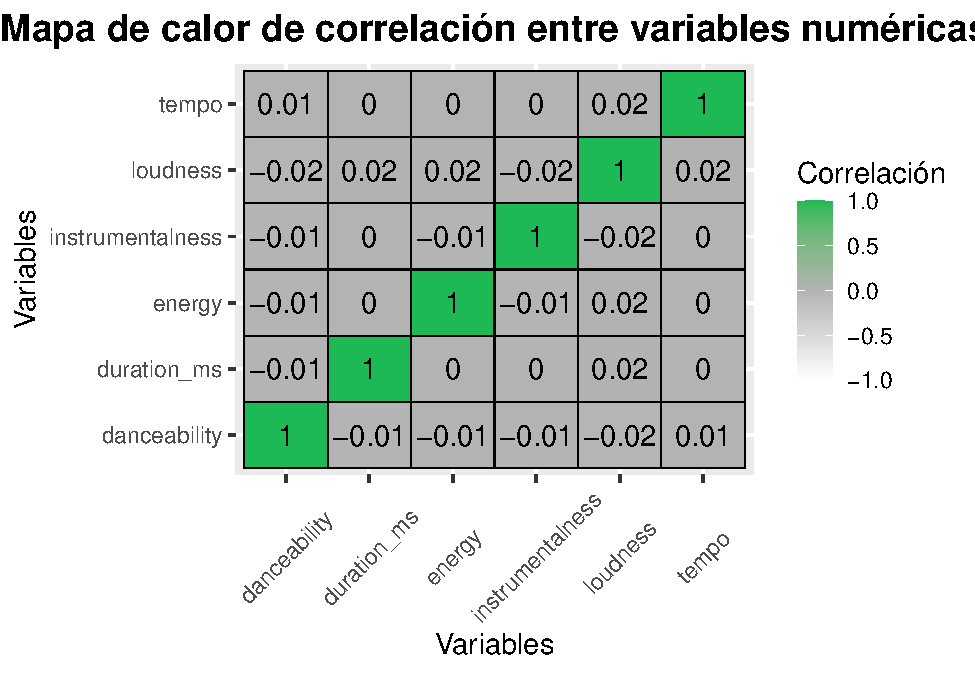
\includegraphics[width=0.9\linewidth,]{informe_files/figure-latex/unnamed-chunk-1-1} \end{center}

Descripción\\

\chapter{Análisis de Resultados}

\{\small Este capítulo presenta los resultados obtenidos al aplicar las
metodologías descritas en el capítulo anterior, así como del análisis
estadístico descriptivo de las variables estudiadas y las ventajas y
desventajas al aplicar dichos tests.\}

\section{Presentación de resultados 1}

Descripción\\

\section{Presentación de resultados 2}

Descripción\\

\section{Presentación de resultados n}

Descripción\\

\chapter{Conclusiones y Recomendaciones}

\textbf{1.-} Conclusion 1 del trabajo de investigación.\\

\textbf{Recomendación} Recomendación 1 del trabajo de investigación.\\

\textbf{2.-} Conclusion 2 del trabajo de investigación.\\

\textbf{Recomendación} Recomendación 2 del trabajo de investigación.\\

\textbf{n.-} Conclusion n del trabajo de investigación.\\

\textbf{Recomendación} Recomendación n del trabajo de investigación.\\

\appendix
\renewcommand{\thechapter}{\Alph{chapter}}

\chapter{Anexo A}

\chapter{Anexo B}

\chapter{Anexo C}

%%%%%%%%%%%%%%%%%%%%%%%%%%%%%%%%%%%%%%%%%%%%%%%%%%%%%
%                   REFERENCIAS                     %
%%%%%%%%%%%%%%%%%%%%%%%%%%%%%%%%%%%%%%%%%%%%%%%%%%%%%
% Mantenemos la estructura natbib de tu plantilla
\renewcommand{\bibname}{Lista de Referencias}
\bibliographystyle{apalike} 
\bibliography{bibliografia.bib} 

%%%%%%%%%%%%%%%%%%%%%%%%%%%%%%%%%%%%%%%%%%%%%%%%%%%%%
%                   APÉNDICES                       %
%%%%%%%%%%%%%%%%%%%%%%%%%%%%%%%%%%%%%%%%%%%%%%%%%%%%%

\end{document}
